\chapter{An'alisis de la planilla de notas}
\label{capitulotres}
El plantel docente de la Facultad de Ciencias y Tecnolog'ia de la Universidad Mayor de San Sim'on utiliza la p'agina del Sistema de Apoyo a la Gesti'on Acad'emica y Administrativa el c'ual tiene una secuencia de pasos  para descargar y publicar la planilla de notas. Para reconocer y modificar la planilla de notas se utiliza, la aplicaci'on del transcriptor.exe la  c'ual tiene diferentes casos, dependiendo de la estructura de la planilla de notas.

\section{Entrevista}
La siguiente entrevista se realizo al \textit{Ing. Cristian Lazarte}, responsable del proyecto Transcriptor.exe en la UPSI \footnote{UPSI-Unidad de Provisi'on de Servicios de Informaci'on} de la UMSS \footnote{UMSS-Universidad Mayor de San Sim'on}. A continuaci'on se muestra los resultados de la entrevista en los siguientes puntos.
\begin{itemize}
\item Explicaci'on de la estructura de planilla de notas, el archivo sis:
\begin{itemize}
\item El c'odigo de la UPSI.
\item El c'odigo de template define la estructura que utiliza el Transcriptor.exe.
\item En el template el ARB son valores permitidos, para A de aprobado, R reprobado y B abandonado.
\item Los datos del grupo est'an definidos en el template y las restricciones de las calificaciones.
\end{itemize}
 
\item Mencionamos  algunos de los aspectos importantes y/o limite que considera a la hora de modificar la planilla de notas en el transcriptor.exe.
\begin{itemize}
\item Modificar las notas se debe mostrar en grillas.
\item Los estados para volver atras.
\item Cuando modifica la lista de estudiantes, no debe permitir cerrar sin guardar.
\item Habilitar la 2da opci'on y tomar en cuenta el mayor entre la 1ra y 2da opci'on.
\item En el enter, ir al siguiente dato para introducir.
\item Analizar la visualizaci'on en el dispositivo m'ovil.
\end{itemize}
\end{itemize}
La entrevista ha proporcionado la comprensi'on  de la estructura y la funcionalidad al modificar la planilla de notas.

\section{Diagrama de proceso de llenar la planilla de notas}
Los procesos de llenar la planilla de notas tiene los siguientes pasos:  descargar la planilla de notas, modificar la planilla de notas y adjuntar la planilla de notas. Se explica con mas detalle en el c'apitulo \ref{capitulocinco} en la secci'on de \ref{Doc:Interfaz}.\\ 
La uni'on de los proceso se representa en un diagrama general como se muestra en la  figura \ref{fig:DiagramaF}
\begin{figure}[H]
\centering
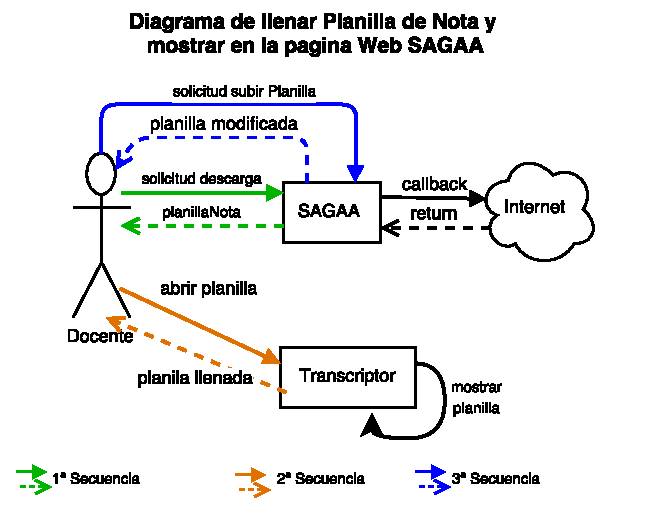
\includegraphics[width=0.4\textwidth]{SGeneralLlenaN.pdf}
\captionsetup{justification=centering, margin=2cm}
\caption{Diagrama de la funcionalidad de llenar y mostrar las notas, en la p'agina del SAGAA Fuente: Elaboraci'on propia}
\label{fig:DiagramaF}
\end{figure}

A continuaci'on se explica la funcionalidad del llenado de planilla de notas de la p'agina SAGAA\footnote{SAGAA-Sistema de Apoyo a la Gesti'on Acad'emica y Administrativa} y la herramienta del transcriptor.exe.


\section{Sistema de apoyo a la gesti'on acad'emica y administrativa}
El sistema de apoyo a la gesti'on acad'emica y administrativa tiene alrededor de 10 a'nos proporcionando el servicio de gestionar la informaci'on acad'emica de pre-grado de los estudiantes.

La funcionalidad de la informaci'on acad'emico de pre-grado tiene los siguientes procesos: 
\begin{itemize}
\item Llenar curriculum.
\item Publicar y modificar avisos.
\item Publicar y modificar las materias.
\item Descargar la planilla de notas.
\item Habilitar la planilla de notas.
\item Ver estudiantes habilitados.
\item Administrador de archivos y manual.
\end{itemize}


Para el presente proyecto se ha utilizado la funcionalidad de modificar la planilla de notas: descargar y habilitar la planilla de notas. Las cuales son.

\subsection{Funcionalidad de modificar la planilla de notas}
La funcionalidad de modificar la planilla de notas tiene los siguientes procesos  descargar, modificar y adjuntar la planilla de notas. A continuaci'on se explican. 

\subsection{Los pasos para descargar la planilla de notas}
\label{PasosDescargar}
Para realizar la descarga de la planilla de notas se explican en los siguientes pasos:
\begin{enumerate}[\bfseries P{a}so 1:]
\item Primeramente, se debe escribir la direcci'on de la p'agina en el navegador: \url{http://pruebas.fcyt.umss.edu.bo/sagaa}. Despu'es se debe acceder al link \textbf{Ingresar al sistema}, debe ingresar su cuenta de usuario y contrase'na as'i como se muestra en la figura \ref{fig:Paso2P}.
%\begin{figure}[H]
%\centering
%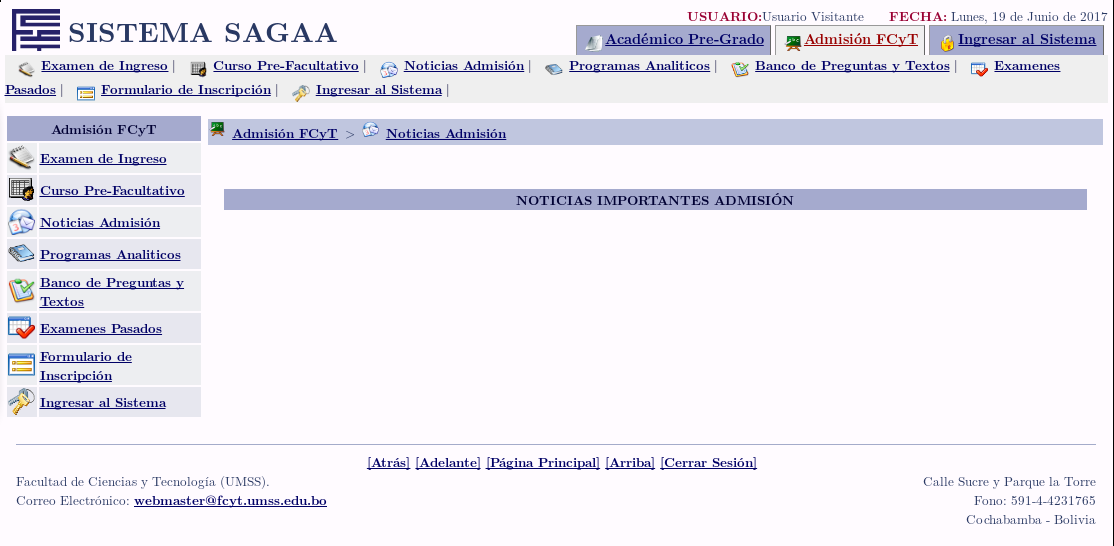
\includegraphics[width=0.5\textwidth]{pagS.png}
%\captionsetup{justification=centering, margin=2cm}
%\caption{Inicio de p'agina del SAGAA Fuente: Proporcionado por la UPSI de la FCYT}
%\label{fig:Paso1P}
%\end{figure}

%\item \textbf{Paso 2:} Hacer click en el link \textit{Ingresar al sistema}, debe ingresar su cuenta de usuario y contrase'na, se muestra en la figura \ref{fig:Paso2P}.
\begin{figure}[H]
\centering
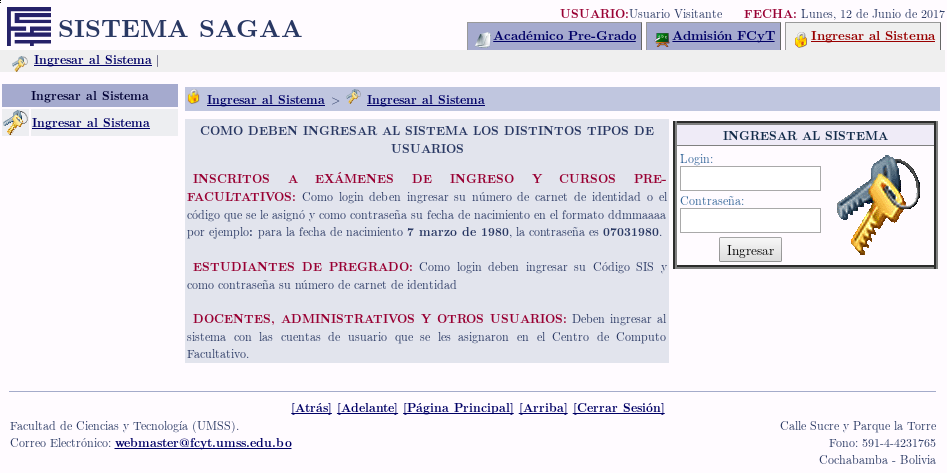
\includegraphics[width=0.5\textwidth]{pagS1.png}
\captionsetup{justification=centering, margin=2cm}
\caption{Iniciar sesi'on en la p'agina del SAGAA Fuente: Proporcionado por la UPSI de la FCYT}
\label{fig:Paso2P}
\end{figure}

\item Elegir el m'enu de usuario \textbf{Acad'emico Pre-Grado} en la figura \ref{fig:Paso3P}.
\begin{figure}[H]
\centering
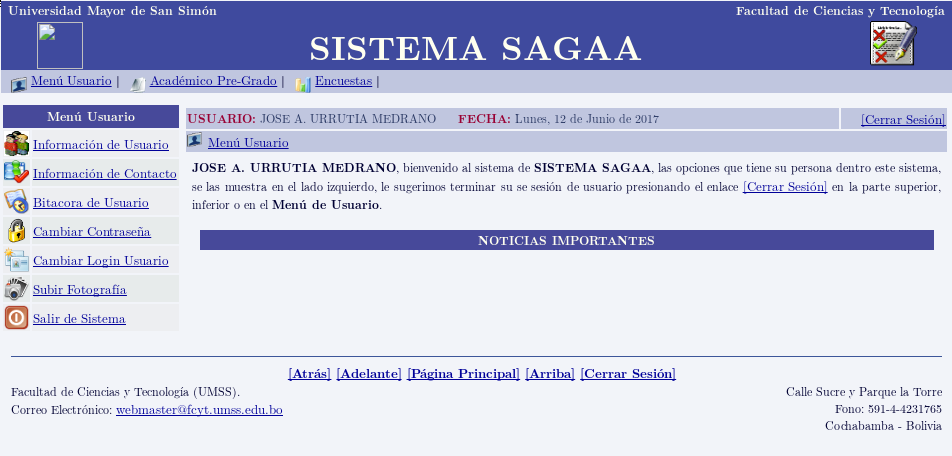
\includegraphics[width=0.5\textwidth]{pagS2.png}
\captionsetup{justification=centering, margin=2cm}
\caption {Elegir men'u Ac'ademico Pre-Grado Fuente: Proporcionado por la UPSI de la FCYT}
\label{fig:Paso3P}
\end{figure}

\item Elegir el men'u la opci'on \textit{" Descargar Planilla de Notas"} de  la figura \ref{fig:Paso4P}.
\begin{figure}[H]
\centering
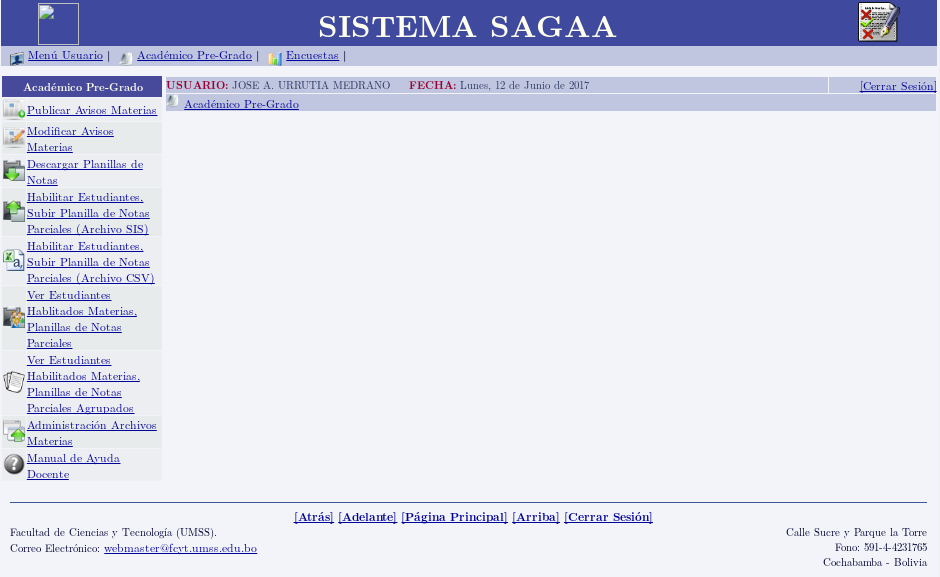
\includegraphics[width=0.5\textwidth]{pagS3.png}
\captionsetup{justification=centering, margin=2cm}
\caption{Elegir la opci'on descargar la planilla de notas Fuente: Proporcionado por la UPSI de la FCYT}
\label{fig:Paso4P}
\end{figure}

\item En la figura \ref{fig:Paso5P} se debe seleccionar la gesti'on de la lista de opciones \textbf{Seleccionar gesti'on}.
\begin{figure}[H]
\centering
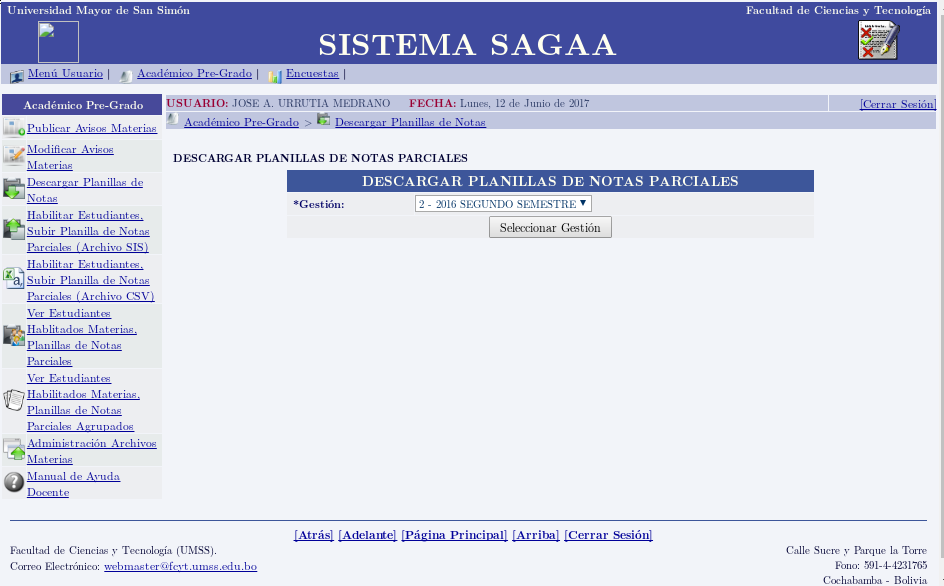
\includegraphics[width=0.5\textwidth]{pagS4.png}
\captionsetup{justification=centering, margin=2cm}
\caption{Opci'on de gesti'on, Fuente: Proporcionado por la UPSI de la FCYT}
\label{fig:Paso5P}
\end{figure}

\item Seleccionar el icono de descarga de la lista de carrera para \textit{Descargar la  planilla de notas}, como se muestra en la figura \ref{fig:Paso6P}.
\begin{figure}[H]
\centering
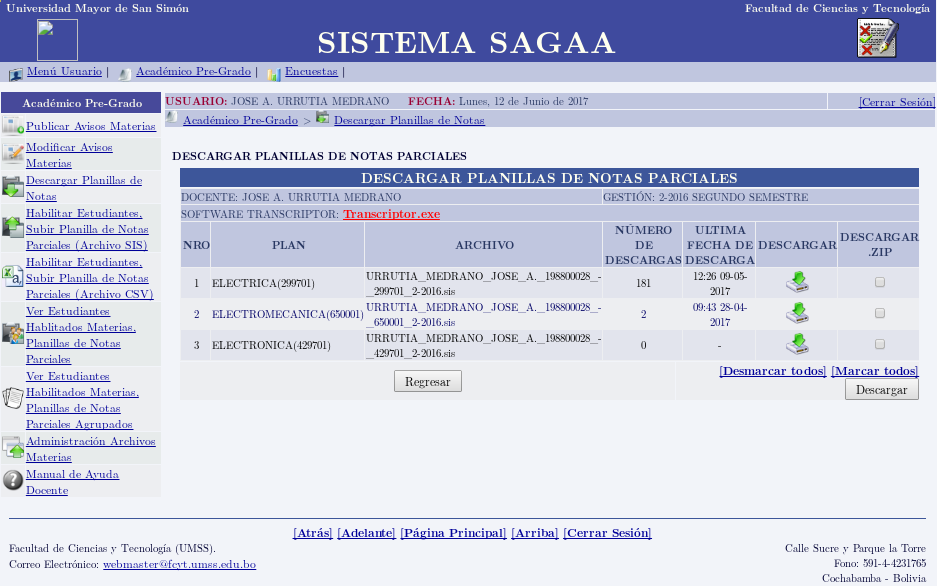
\includegraphics[width=0.5\textwidth]{pagS5.png}
\captionsetup{justification=centering, margin=2cm}
\caption{Elegir la descarga de una planilla de notas, Fuente: Proporcionado por la UPSI de la FCYT}
\label{fig:Paso6P}
\end{figure}
\end{enumerate}
Finalmente, el documento de planilla de notas debe llenar las notas y despu'es realizar el proceso de publicaci'on de la planilla de notas.

\subsection{Los pasos para publicar la planilla de notas}
Para publicar la planilla de notas, se realiza el paso 1 de \textbf{Ingressar al sistemas} y el paso 2 elegir el men'u \textbf{Acad'emico Pre-Grado} de la secci'on  \ref{PasosDescargar} de descargar la planilla de notas , despu'es se debe realizar los siguientes pasos:
\begin{enumerate}[\bfseries P{a}so 1:]
\item Elegir el men'u la opci'on, \textbf{Habilitar estudiantes, subir Planilla de Notas Parciales (Archivo SIS)}, como se muestra en la figura \ref{fig:Paso1PS}.
\begin{figure}[H]
\centering
\captionsetup{justification=centering, margin=2cm}
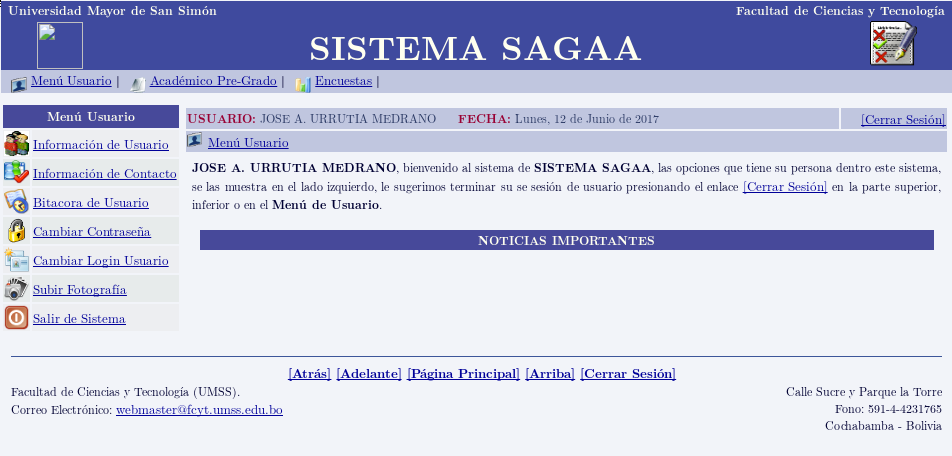
\includegraphics[width=0.6\textwidth]{pagS2.png}
\caption{Paso 1: Opci'on de habilitar estudiantes Fuente: Proporcionado por la UPSI de la FCYT}
\label{fig:Paso1PS}
\end{figure}

\item En la figura \ref{fig:Paso2PS} se adjunta el archivo y se selecciona la gesti'on de la lista de opciones, despu'es de hacer click en \textbf{Subir Archivo}
\begin{figure}[H]
\centering
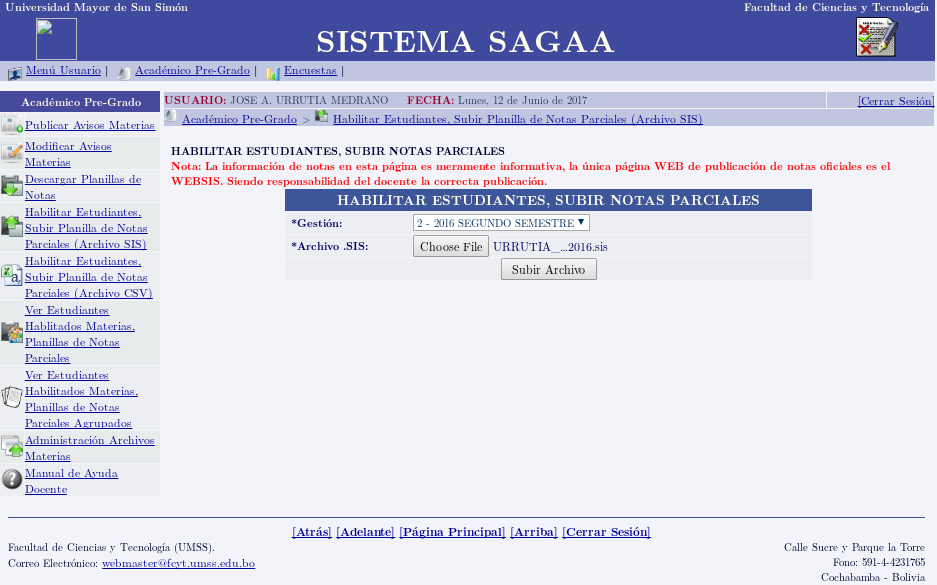
\includegraphics[width=0.5\textwidth]{pagS7.png}
\captionsetup{justification=centering, margin=2cm}
\caption{Paso 2: Opci'on de adjuntar el archivo seleccionado Fuente: Proporcionado por la UPSI de la FCYT}
\label{fig:Paso2PS}
\end{figure}

\item Seleccionar el grupo para adjuntar la planilla de notas y por ultimo click en \textbf{Finalizar Operaci'on} como se muestra en la figura\ref{fig:Paso3PS}.
\begin{figure}[H]
\centering
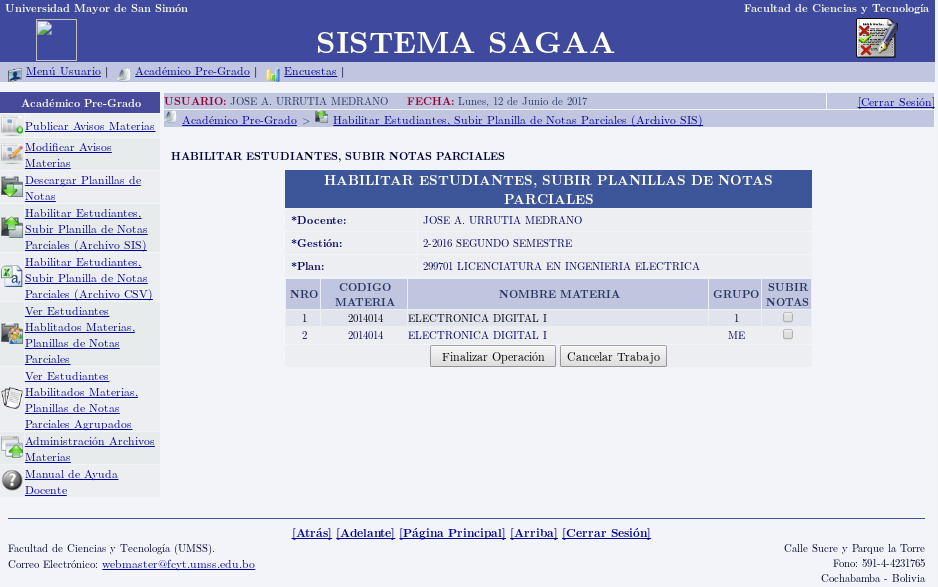
\includegraphics[width=0.5\textwidth]{pagS8.png}
\captionsetup{justification=centering, margin=2cm}
\caption{Paso 3: Subir planilla de notas por grupo Fuente: Proporcionado por la UPSI de la FCYT}
\label{fig:Paso3PS}
\end{figure}
\end{enumerate}

Al finalizar, se muestra el mensaje \textit{Finalizo la  habilitaci'on de estudiantes y la planilla de notas} y accede nuevamente al paso 1.

\subsection{Las restricciones de la p'agina del SAGAA}
Para concluir con el an'alisis de la p'agina del SAGAA se debe tomar en cuenta las siguientes restricciones: 
\begin{enumerate}
\item Solo permite subir planilla de notas con extensi'on sis.
\item Se debe estar conectado a internet para realizar el adjuntar o descargar la planilla de notas.
\end{enumerate}

\section{El transcriptor}
El trascriptor es un programa ejecutable tiene la funcionalidad de modificar la planilla de notas. Previamente, se descarga el documento de planilla de notas de la p'agina del SAGAA \footnote{SAGAA-Sistema de Apoyo a la Gesti'on Acad'emica y Administrativa}. El creador el  Lic. Cristian Lazarte,  qui'en actualmente trabaja en la UPSI \footnote{UPSI-Unidad de Provisi'on de Servicios de Informaci'on} realizando mantenimiento a dicha aplicaci'on.


\subsection{La funcionalidad de la aplicaci'on del transcriptor}
La funcionalidad del transcriptor es llenar la planilla de notas las cuales se describen en los siguientes pasos.
\begin{enumerate}[\bfseries P{a}so 1:]
\item Primeramente seleccionar el bot'on \textbf{Abrir} como se observa en el c'irculo azul. En segundo lugar se busca la ubicaci'on de la planilla de notas, como se observa en la figura \ref{fig:Paso1T}.
\begin{figure}[H]
\centering
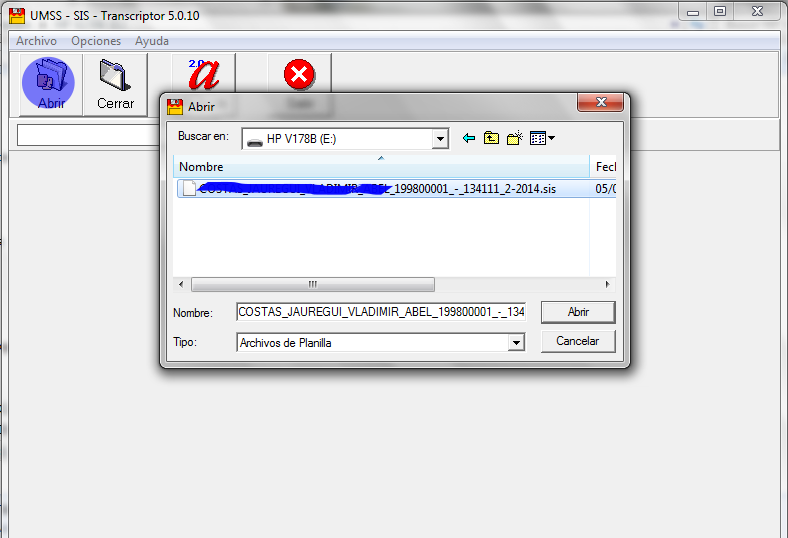
\includegraphics[width=0.5\textwidth]{t1.png}
\captionsetup{justification=centering, margin=2cm}
\caption{Buscar planilla de notas  del Transcriptor Fuente: Proporcionado por el MEMI}
\label{fig:Paso1T}
\end{figure}

\item Seleccionar un grupo y hacer click en el c'irculo azul, en el bot'on \textbf{Editar}, se representa en la figura \ref{fig:Paso2T}.
\begin{figure}[H]
\centering
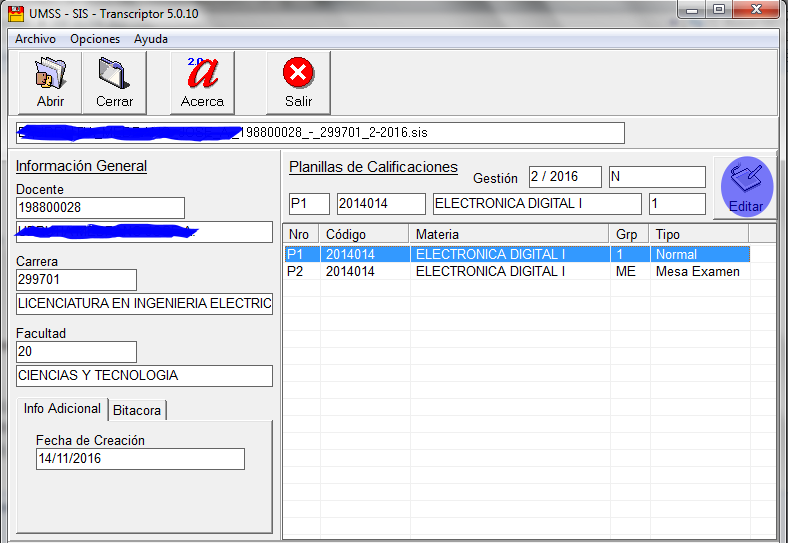
\includegraphics[width=0.5\textwidth]{t2.png}
\captionsetup{justification=centering,margin=2cm}
\caption{Buscar planilla de notas Fuente: Proporcionado por el MEMI}
\label{fig:Paso2T}
\end{figure}

\item En el c'irculo rosado se debe llenar las notas de forma ordenada, como se tiene en la figura \ref{fig:Paso3T}.
\begin{figure}[H]
\centering
\captionsetup{justification=centering,margin=2cm}
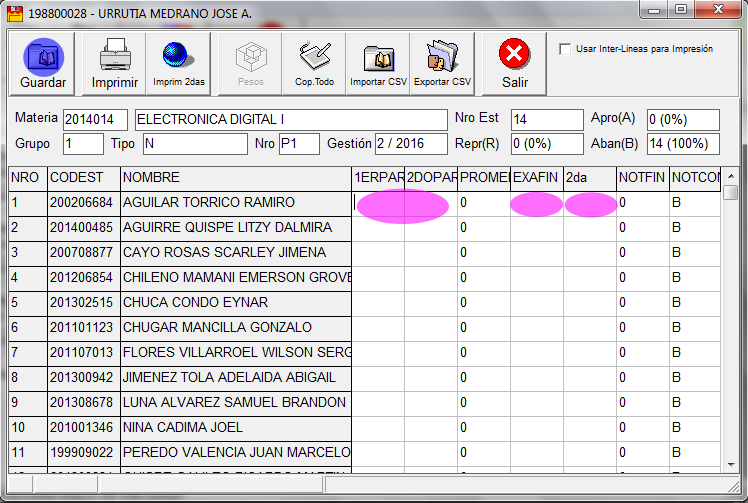
\includegraphics[width=0.6\textwidth]{t3.png}
\caption{Lista de estudiantes, Fuente: Proporcionado por el MEMI}
\label{fig:Paso3T}
\end{figure}
 
\item Guardar la planilla de notas y hacer click en el bot'on \textbf{Guardar} para cerrar la ventana y guardar los datos en el archivo de planilla de notas como se muestra en la figura \ref{fig:Paso3T}.
\end{enumerate}

Desp'ues de concluir con descargar y  adjuntar la planilla de notas, se modifica la planilla de notas con el transcriptor.exe.

\subsection{Detalle del Transcriptor}
El transcriptor interpreta los datos de la planilla de notas que se encuentra con la extensi'on sis, como se muestra en los siguiente casos a continuacio'on en la figura \ref{fig:Caso1T}.
\begin{enumerate}[\bfseries P{a}so 1:]
\item Mostrar los datos de la informaci'on general y la lista de materias, como se muestra en la figura \ref{fig:Caso1T}
\begin{figure}[H]
\centering
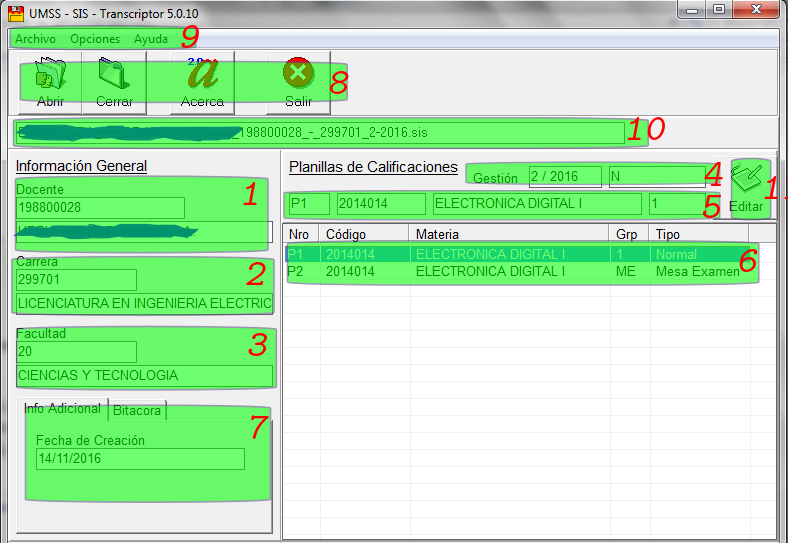
\includegraphics[width=0.6\textwidth]{td2.png}
\captionsetup{justification=centering,margin=2cm}
\caption{Detalle de la lista de grupo Fuente: Proporcionado por el MEMI}
\label{fig:Caso1T}
\end{figure}

Se divide en las siguientes partes, las cuales est'an enumeradas seg'un el detalle:
\begin{enumerate}
\item Los datos del docente: el c'odigo, el nombre y apellido.
\item Los datos de la carrera: el c'odigo y nombre.
\item Los datos de la facultad: el c'odigo y nombre.
\item El dato de la gesti'on.
\item Los datos del grupo: el c'odigo, nombre, c'odigo de reconocimiento y n'umero de grupo.
\item La lista de grupo: el n'umero, c'odigo, nombre, identificador y tipo.
\item La informaci'on adicional de una bitacora de la fecha de creaci'on y bit'acora del archivo.
\item En el men'u del n'umero 8 tiene los eventos  los cuales son: abrir, cerrar, acerca y salir.
\item En el men'u del n'umero 9 consta de los eventos: archivo, opciones y ayuda.
\end{enumerate}

\item Mostrar la lista de estudiantes, como se muestra en la figura \ref{fig:Caso2T}.
\begin{figure}[H]
\centering
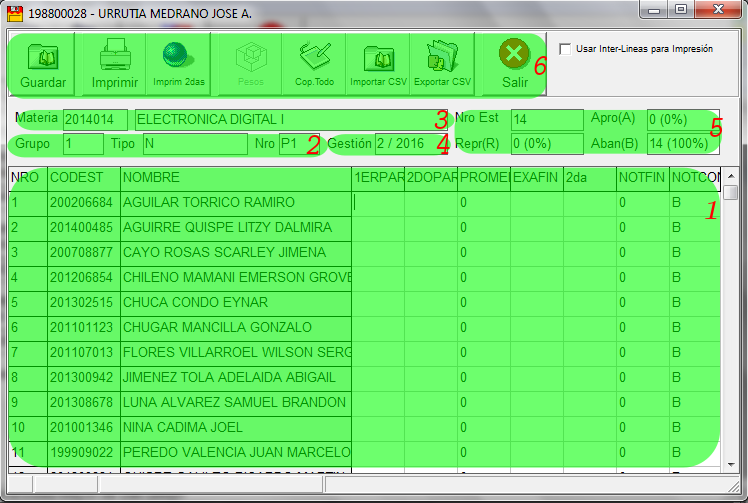
\includegraphics[width=0.6\textwidth]{td3.png}
\captionsetup{justification=centering, margin=2cm}
\caption{Detalle de la lista de estudiantes Fuente: Proporcionado por el MEMI}
\label{fig:Caso2T}
\end{figure}

La lista de estudiantes se divide en las siguientes partes, las cuales est'an enumeradas detalladamente en la siguiente lista:
\begin{enumerate}
\item La lista de estudiantes consta con los siguientes datos: n'umero, c'odigo, nombre, 1er parcial, 2do parcial, promedio, examen final, 2da instancia, nota final y nota contado.
\item Los datos del grupo son: c'odigo de reconocimiento, tipo y n'umero de grupo.
\item Los datos de la materia son: el c'odigo y nombre.
\item El dato de gesti'on.
\item En los datos extra de los estudiantes estan : la cantidad, porcentaje de reprobado, aprobado y abandonado.
\item La lista de men'u son guardar, imprimir, imprimir 2da instancia, pesos, copia todo, importar csv, exportar csv y salir.
\end{enumerate}
\end{enumerate}

\subsection{Las restricciones del transcriptor}
La aplicaci'on del transcriptor, seg'un el detalle y la funcionalidad, tiene las siguientes restricciones:
\begin{enumerate}
\item Se puede usar 'unicamente en el sistema operativo windows.
\item Solo permite abrir archivos con la extensi'on sis.
\item No permite abrir un documento de planilla de notas, si estas da'nado.
\item Controla los datos a ser insertados.
\item Protege la informaci'on del archivo y solo permite modificar la nota del estudiante.
\item Solo permite modificar la planilla de nota por grupo.
\item No permite cerrar la lista de grupos, sin previamente haber guardado.
\end{enumerate}

Despu'es de concluir con el an'alisis del transcriptor, se empieza a analizar el contenido de la planilla de notas que tiene la extensi'on sis.

\section{La planilla de notas}
El documento de la planilla de notas es un  est'andar que utiliza la UMSS\footnote{UMSS-Universidad Mayor de San Sim'on} para la modalidad de calificaci'on de las diferentes carreras. Para explicar la utilidad de la planilla de notas se divide en  la informaci'on y la estructura de la planilla de notas.


% aqui me quede
\subsection{La informaci'on de la planilla de notas}
La informaci'on se divide en datos academicos, la estructura del formato de los grupos, la estructura de los grupos y estructura de la informaci'on del estudiante. En el siguiente p'arrafo se explicara.
\begin{enumerate}
\item  Los datos academicos se explica en cada lin'ea del documento de la planilla de notas, la c'ual tiene la siguiente estructura.
\begin{verbatim}
PCD5.0 //codigo inicio
2719  //codigo fin
09/08/2016 //fecha de creacion
09/08/2016 //fecha de creacion
198800028 //codigo docente
URRUTIA MEDRANO JOSE A.//nombre y apellido docente
299701//codigo carrera
LICENCIATURA EN INGENIERIA ELECTRICA //nombre carrera
2016// gestion
1 //numero gestion
Primer Semestre //literal del semestre
20 //codigo facultad
CIENCIAS Y TECNOLOGIA //nombre facultad
11 //codigo UPSI
UPSI nombre Upsi
263 //tipo de template
tecno //carrera de template
26	//nota maxima para el template
\end{verbatim}
\item La estructura del formato de grupos se explica en forma horizontal del documento de planilla de notas.\\
\begin{verbatim}
\\a,b   ,c ,d,e  ,f,g ,h ,i,j,k   
1,NUMERO,RD,0,100,,NRO,38,N,N,NONE
.........
10,NOTCON,RD,0,100,ARB,NOTCON,50,N,N,ERES
\end{verbatim}
\begin{enumerate}
\item 1 es el orden de la fila.
\item NUMERO es identificador de la  etiqueta ordenado por fila.
\item RD o WR permiso de lectura o escritura.
\item 0 es el inicio del rango de datos.
\item 100 o 51  es el final del rango de datos.
\item A o R o B  es el valor permitido.
\item NRO nombre de la etiqueta ordenado por fila.
\item 38 o 72 o 230 o 52 o 50 ancho de la columna.
\item N para habilitar si tiene nota final.
\item N para habilitar si tiene segunda instancia.
\item NONE palabra reservado.
\end{enumerate}
La estructura del formatos de los grupos depende del formato de calificaci'on es por lo c'ual el grupo normal tiene 10 columnas y el grupo mesa tiene 7 columnas.

\item La estructura del formato de los grupos se divide por la coma se explican a continuaci'on de manera secuencial.\\
Detalle grupo normal:
\begin{verbatim}
\\a, b,   ,c, d 				  ,e  , f ,g,h ,i ,j,k,l,m 	
P1,2014014,1,ELECTRONICA DIGITAL I,263,100,0,50,50,0,0,0,0
P2,2014014,ME,ELECTRONICA DIGITAL I,263,100,0,50,50,0,0,0,0
\end{verbatim}
\begin{enumerate}
\item P1 o P2 es el c'odigo grupo.
\item 2014014 es el c'odigo de la materia.
\item 1 o ME es el tipo de grupo.
\item ELECTRONICA DIGITAL I es el nombre de la materia.
\item 263 es el tipo de template.
\item 100 es el peso global de T1, T2 y T3.
\item 0 es el peso del examen final.
\item 50 es el T1.
\item 50 es el T2.
\item 0 es el T3.
\item 0 es el P1
\item 0 es el P2.
\item 0 es el P3.
\end{enumerate}
Los datos que empieza con la letra P son los parciales y los datos que empieza  con la letra T son los trabajos.
\item La estructura de la informaci'on del estudiante    se divide en grupo normal y mesa como se muestra a continuaci'on.
\begin{enumerate}
\item Lista de estudiantes de grupo normal tiene 10 columnas como se muestra en la siguiente linea del documento:
\begin{verbatim}
1,200206684,AGUILAR TORRICO RAMIRO,,,,,,,
\end{verbatim}
La estructura de la informaci'on del estudiante se explica de manera secuencial los cuales son: 1 es NRO, 200206684 es COD, AGUILAR TORRICO RAMIRO es NOMEST, vacio es 1ERPAR , vacio es 2DOPAR, vacio es PROMED, vacio es EXAFIN, vacio es 2da, vacio es NOTFIN y vacio es NOTCON.
\item Lista de estudiantes del grupo mesa tiene 7 columnas, seg'un la siguiente linea del documento:
\begin{verbatim}
1,201209060,CALIZAYA MAMANI GAITH EFRAIN,20,,20,R
\end{verbatim}
La lista de estudiantes se desarrollan de forma ordenada estas son: 1 es NRO, 200206684 es COD, CALIZAYA MAMANI GAITH EFRAIN es NOMEST, 20 es 1RAOPC, vacio es 2DAOPC, 20 es NOTFIN y vacio es NOTCON.
\end{enumerate}
\end{enumerate}

\subsection{La estructura de la planilla de notas}
La estructura de la planilla de notas tiene una estructura de etiqueta de inicio y final el c'ual divide a la informaci'on en una manera organizada para el reconocimiento del transcriptor.exe. A continuaci'on se explica el orden de la estructura de la planilla de notas.
\begin{verbatim}
<pcd>(inicio documento)
<head>(inicio cabecera)
<info>(inicio Informacion)
</info> (fin Informacion)
<columna> (inicio columna)
<template> (inicio template)
<normal> (inicio normal)
</normal>(fin normal)
<me>(inicio mesa)
</me>(fin mesa)
</template>(fin template)
</column>(fin columna)
<group>(inicio de grupo)
  <normal>(inicio de grupo normal)
  </normal>(fin de grupo normal)
  <me>(inicio de grupo mesa)
  </me>(fin de grupo mesa)
</group>(fin de grupo mesa)
</head>(fin de cabecera)
<body>(inicio cuerpo)
<gradelist>(inicio de lista)
<P1>(inicio materia tipo)
</P1>(fin materia tipo)
<P2>(inicio materia tipo)
</P2>(fin materia tipo)
</gradelist>(fin de lista)
/body>(fin cuerpo)
</pcd>(fin documento)
\end{verbatim}

\subsection{Las restricciones de la planilla de notas}
La planilla de notas es un archivo con extensi'on sis que tiene las siguientes restricci'on:
\begin{enumerate}
\item No se debe cambiar la extensi'on.
\item No se debe alterar la estructura del archivo en caso contrario no sera reconocido por la aplicaci'on del transcriptor.exe.
\end{enumerate}                

En conclusi'on  se puede notar que  la funcionalidad de modificar la planilla de notas tiene 3 procesos en los cuales se utilizan las siguientes aplicaciones: la p'agina del SAGAA\footnote{SAGAA - Sistema de Apoyo a la Gesti'on Acad'emica y Administrativa} y el transcriptor.exe. Tomando en cuenta que cada uno tiene su respectiva restricci'on es por este motivo que se elige esta misma como una herramienta de prueba. 